% Generated by book/tools/notebook_to_tex.py. Do not edit by hand.

\chapter[한국어 BERT 다중 라벨 분류 (Korean Multi-label Classification)]{한국어 BERT 다중 라벨 분류 (Korean Multi-label Classification)}

\label{ch:17}

\markboth{한국어 BERT 다중 라벨 분류 (Korean Multi-label Classification)}{한국어 BERT 다중 라벨 분류 (Korean Multi-label Classification)}

\chaptermeta{17_ko_multilabel/17_ko_multilabel.ipynb}{https://colab.research.google.com/github/yoon-gu/neuqes-101/blob/master/17_ko_multilabel/17_ko_multilabel.ipynb}{KLUE-YNAT 결합 샘플로 한국어 BERT의 라벨별 sigmoid와 BCE를 학습}



\index{1Korean BERT@Korean BERT}

\index{1KLUE BERT@KLUE-BERT}

\index{1klue bert base@klue/bert-base}

\index{1KLUE YNAT@KLUE-YNAT}

\index{1multi label classification@multi-label classification}

\index{1BCEWithLogitsLoss@BCEWithLogitsLoss}

\index{1multi hot label@multi-hot label}

\index{1per label sigmoid@per-label sigmoid}

\index{1hamming loss@hamming\_loss}

\index{1micro F1@micro F1}

\index{1macro F1@macro F1}

\index{1threshold sweep@threshold sweep}

\index{1co occurrence matrix@co-occurrence matrix}

\index{0한국어 BERT@한국어 BERT}

\index{0한국어 다중 라벨 분류@한국어 다중 라벨 분류}

\index{0멀티핫@멀티핫}

\index{0라벨별 시그모이드@라벨별 시그모이드}

\index{0라벨별 BCE@라벨별 BCE}

\index{0임계값 탐색@임계값 탐색}

\index{0공동 활성@공동 활성}

\index{0뉴스 다중 라벨@뉴스 다중 라벨}

\index{1problem type multi label classification@problem\_type="multi\_label\_classification"}

\index{1sigmoid probability@sigmoid probability}

\index{1multi hot vector@multi-hot vector}

\index{1precision recall fscore support@precision\_recall\_fscore\_support}

\index{1classification report@classification\_report}

\index{1roc auc score@roc\_auc\_score}

\index{1seaborn FacetGrid@seaborn.FacetGrid}

\index{1threshold 0 5@threshold=0.5}

\index{1pos weight@pos\_weight}

\index{1synthetic multi label data@synthetic multi-label data}

\index{1active label count@active label count}

\index{1conditional probability@conditional probability}

\index{0라벨별 확률@라벨별 확률}

\index{0활성 라벨 수@활성 라벨 수}

\index{0합성 다중 라벨 데이터@합성 다중 라벨 데이터}

\index{0카테고리별 임계값@카테고리별 임계값}

\index{0조건부 확률@조건부 확률}

\index{0불균형 가중치@불균형 가중치}



\section{변화추적표}

\begin{booktable}{17장 변화추적표}{tab:ch17-01}
\begin{adjustbox}{max width=\textwidth}
\begin{tabular}{@{}lllllll@{}}
\toprule
Ch & 모델 & 토크나이저 & 데이터 & Output Head & Activation & Loss \\
\midrule

13 & DistilBERT & WordPiece (영어) & Yelp + 항목 키워드 합성 & \inlinecode{Linear(H,\ 5)} & sigmoid (per-label) & \inlinecode{BCEWithLogitsLoss} (per-label) \\
15 & klue/bert-base & WordPiece (한국어) & NSMC binary & \inlinecode{Linear(H,\ 2)} & softmax & \inlinecode{CrossEntropyLoss} \\
16 & klue/bert-base & 같음 & KLUE-YNAT (뉴스 7분류) & \inlinecode{Linear(H,\ 7)} & softmax & \inlinecode{CrossEntropyLoss} \\
\textbf{17 \(\leftarrow\) 여기} & klue/bert-base & 같음 & \textbf{KLUE-YNAT 합성 multi-label (두 헤드라인 결합)} & \inlinecode{Linear(H,\ 7)} & \textbf{sigmoid (per-label)} & \textbf{\inlinecode{BCEWithLogitsLoss} (per-label)} \\
18 (다음) & klue/bert-base & 같음 & KLUE-YNAT 합성 multi-label + 라벨 개수 보조 & \inlinecode{Linear(H,\ 7)} 메인 + \inlinecode{Linear(H,\ 1)} 보조 & sigmoid + 없음 & \texttt{BCE(per-label)\ +\ λ·MSE} \\
\bottomrule
\end{tabular}
\end{adjustbox}
\end{booktable}

전체 장 표는 \href{https://github.com/yoon-gu/neuqes-101\#챕터별-변화추적표}{루트 README.md}를 참고하세요.



\section{변경점: \ref{ch:16}장 대비}

\begin{booktable}{17장 변경점 요약}{tab:ch17-02}
\begin{adjustbox}{max width=\textwidth}
\begin{tabular}{@{}lll@{}}
\toprule
축 & \ref{ch:16}장 (한국어 multi-class) & \ref{ch:17}장 (한국어 multi-label) \\
\midrule

\textbf{Task} & 7-클래스 \emph{single-label} (서로 배타적) & \textbf{7-라벨 \emph{multi-label}} (동시 활성 가능) \(\leftarrow\) \emph{유일한 변화} \\
\inlinecode{num\_labels} & 7 & \textbf{7} (그대로!) \\
\inlinecode{problem\_type} & \inlinecode{"single\_label\_classification"} & \textbf{\inlinecode{"multi\_label\_classification"}} \(\leftarrow\) BCE 자동 매핑 \\
Activation & softmax (합=1 강제) & \textbf{per-label sigmoid} (각각 독립 0-1) \\
Loss & \inlinecode{CrossEntropyLoss} & \textbf{\inlinecode{BCEWithLogitsLoss}} per-label \\
라벨 형식 & int 스칼라 (0-6) & \textbf{multi-hot float 7차원 \texttt{{[}0,\ 1,\ 0,\ 0,\ 0,\ 1,\ 0{]}}} \\
데이터 & KLUE-YNAT 원본 헤드라인 & \textbf{두 헤드라인 결합 \(\to\) 두 카테고리 union} \\
평가 metric & accuracy + macro F1 + AUC OvR & \textbf{hamming loss + micro/macro F1 + per-label F1 + macro AUC} \\
모델 본체 / 토크나이저 / hyperparams & (모두 동일) & (모두 동일) \\
\bottomrule
\end{tabular}
\end{adjustbox}
\end{booktable}

\begin{quote}
\textbf{변경점 한 가지 원칙} --- Phase 2 안에선 \emph{task 차원} (single-label \(\to\) multi-label) 만 바뀝니다. 한국어 셋업·hyperparams 는 \ref{ch:16}장과 \emph{완전히 같음}. 모델 아키텍처조차 \inlinecode{Linear(H,\ 7)} 그대로 --- \inlinecode{problem\_type} 한 줄과 라벨 \emph{형식} 만 바뀝니다.
\end{quote}

\subsection{같은 7차원 출력을 두 가지로 해석}

\ref{ch:16}장과 \ref{ch:17}장의 모델은 둘 다 \inlinecode{Linear(768,\ 7)} 헤드를 가집니다. 차이는 \emph{그 7개 숫자를 어떻게 읽는가}:

\begin{itemize}
\tightlist
\item
  \textbf{\ref{ch:16}장 (softmax)}: 7개를 \emph{한꺼번에} 정규화해 합=1 로 만든 뒤 \emph{가장 큰 하나} 를 고름. “이 헤드라인은 7개 카테고리 중 \emph{정확히 하나}”.
\item
  \textbf{\ref{ch:17}장 (per-label sigmoid)}: 7개 각각을 \emph{독립적으로} 0-1 확률로 변환. “이 헤드라인에 각 카테고리가 \emph{각자} 활성됐는가?” --- 여러 개가 동시에 1 일 수 있음.
\end{itemize}



\section{\texorpdfstring{Loss 함수의 변화 --- \inlinecode{CrossEntropyLoss} \(\to\) \inlinecode{BCEWithLogitsLoss} per-label}{Loss 함수의 변화 --- CrossEntropyLoss \textbackslash to BCEWithLogitsLoss per-label}}

\ref{ch:16}장의 multi-class CE 는 \emph{정답 클래스 하나} 의 로그확률만 봤습니다:

\begin{equation}
\label{eq:ch17-01}
L_{\text{CE}} = -\frac{1}{N}\sum_{i=1}^{N}\log \hat p_{i, y_i}
\end{equation}

식~\eqref{eq:ch17-01}은 Cross-Entropy가 K=2에서 BCE와 같은 형태로 정리됨을 보여줍니다.

\ref{ch:17}장은 K=7 개 라벨 각각에 \emph{독립적} BCE 를 적용한 뒤 평균합니다 (\ref{ch:13}장의 식 그대로, 한국어 맥락):

\begin{equation}
\label{eq:ch17-02}
L_{\text{BCE}} = -\frac{1}{N \cdot K}\sum_{i=1}^{N}\sum_{k=1}^{K}\left[ y_{i,k} \log \sigma(z_{i,k}) + (1-y_{i,k}) \log(1-\sigma(z_{i,k})) \right]
\end{equation}

식~\eqref{eq:ch17-02}은 정답 라벨과 예측 확률 사이의 Binary Cross-Entropy를 정의합니다.

각 \(z_{i,k}\) 는 \emph{독립 logit} --- 카테고리 k 가 \emph{얼마나 활성될지} 의 점수, 다른 카테고리와 무관. PyTorch \inlinecode{BCEWithLogitsLoss} 가 7개 위치를 한 번에 처리하지만 수식적으론 7개의 binary BCE 평균입니다.

\textbf{숫자로 감 잡기 (K=7, 정답 multi-hot \(\mathbf{y} = [0, 1, 0, 0, 0, 1, 0]\) --- 경제+스포츠 동시 활성)} --- logit 별 손실 분해:

\begin{booktable}{17장 손실 수치 예시}{tab:ch17-03}
\begin{adjustbox}{max width=\textwidth}
\begin{tabular}{@{}llllll@{}}
\toprule
라벨 & 카테고리 & \(y_k\) & logit \(z_k\) & \(\sigma(z_k)\) & 손실 \(-\log(\cdot)\) \\
\midrule

1 & 경제 & 1 & 3.0 & 0.953 & 0.048 \\
5 & 스포츠 & 1 & 0.5 & 0.622 & 0.474 \\
0 & IT과학 & 0 & -2.0 & 0.119 & 0.127 \\
2 & 사회 & 0 & 1.5 & 0.818 & 1.704 \(\leftarrow\) 자신 있게 틀림 \\
나머지 3개 & (음성) & 0 & -3.0 & 0.047 & 각 0.048 \\
\bottomrule
\end{tabular}
\end{adjustbox}
\end{booktable}

평균 loss = \((0.048 + 0.474 + 0.127 + 1.704 + 0.048 \times 3) / 7 \approx 0.387\).

\textbf{핵심 직관 --- 라벨 사이엔 직접 신호가 없음}: BCE per-label 은 카테고리 k 의 logit 이 카테고리 j 의 정답에서 \emph{직접} 학습 신호를 받지 않습니다. 모델이 카테고리 간 상관을 학습하는 건 \emph{공유 BERT 본체} (모든 라벨이 같은 768-dim CLS 표현에서 옴) 덕분이지 loss 자체엔 라벨 간 결합 항이 없습니다.

\textbf{코드 한 줄 변화} --- \ref{ch:16}장 \(\to\) \ref{ch:17}장:

\Needspace{9\baselineskip}
\begin{lstlisting}
out["labels"] = [int(l) for l in batch["label"]]
problem_type = "single_label_classification"
# → CrossEntropyLoss

out["labels"] = [list(map(float, mh)) for mh in batch["multi_hot"]]
problem_type = "multi_label_classification"
# → BCEWithLogitsLoss per-label
\end{lstlisting}

\subsection{왜 multi-label 은 softmax 로 풀 수 없는가}

softmax 는 출력의 \emph{합 = 1} 을 강제합니다 (\(\sum_k \mathrm{softmax}(z)_k = 1\)). 이는 \emph{서로 배타적} 클래스 (\ref{ch:16}장) 에 자연스럽지만 multi-label 과 충돌합니다.

합성 샘플이 “경제 헤드라인 + 스포츠 헤드라인” 이라 정답이 경제=1, 스포츠=1 일 때:

\begin{itemize}
\tightlist
\item
  \textbf{softmax 모델은 표현 불가}: P(경제)=0.6 이면 나머지 6 라벨 합이 0.4 로 강제 \(\to\) \textquotesingle 스포츠=0.55 동시 활성\textquotesingle{} 이 \emph{수학적으로 불가능}.
\item
  \textbf{per-label sigmoid 모델은 표현 가능}: 각 라벨이 독립이라 P(경제)=0.9 와 P(스포츠)=0.85 가 동시에 자연스러움.
\end{itemize}

즉 task 가 \emph{진짜 multi-label} 이라면 loss/activation 선택이 강제됩니다 (\ref{ch:04}·\ref{ch:13}장에서 본 동일한 논리).



\section{토크나이저 노트}

\ref{ch:16}장과 \emph{완전히 동일} --- \inlinecode{klue/bert-base} 한국어 WordPiece. 토크나이저는 라벨 \emph{형식} (int 스칼라든 multi-hot 벡터든) 에 무관하므로 변화 없음.

\begin{quote}
\textbf{Phase 2 안에서는 토크나이저 고정} --- \ref{ch:15}·\ref{ch:16}장·17·18 모두 같은 한국어 WordPiece. Phase 3 (\ref{ch:19}--\ref{ch:23}장) 에서 비로소 \emph{직접 학습한 워드레벨 토크나이저} 가 등장.
\end{quote}

\subsection{결합 헤드라인 토큰화 예시}

\ref{ch:16}장은 헤드라인 \emph{한 줄} (평균 약 16 토큰) 이었지만, \ref{ch:17}장은 두 헤드라인을 \texttt{{[}SEP{]}} 로 이어붙여 \emph{길이가 약 2배} (평균 약 30 토큰, 최대 41) 가 됩니다. \inlinecode{max\_length=128} 안에 충분히 들어갑니다.

두 문장을 잇는 \texttt{{[}SEP{]}} 토큰은 BERT 가 \emph{문장 경계} 를 인식하는 특수 토큰입니다 --- NSP (Next Sentence Prediction) 사전학습에서 쓰던 그 토큰. 결합 헤드라인에선 두 주제의 경계 역할을 합니다.

\begin{previewBox}{미리보기}
\textbf{다음 장 (\ref{ch:18}장)}: 토크나이저 그대로. 변하는 건 \emph{모델에 보조 헤드} (활성 라벨 \emph{개수} 회귀) 가 추가되고 \emph{loss 에 보조 항} 이 가중합으로 더해지는 점.
\end{previewBox}



\textbf{baseline VRAM} (CUDA 환경에서만 의미 있는 출력 --- Colab T4 기준):



\Needspace{5\baselineskip}
\begin{lstlisting}
!nvidia-smi
\end{lstlisting}

\begin{codeRead}
\textbf{1행}의 \inlinecode{!nvidia-smi}에서는 앞 단계에서 만든 값을 바탕으로 다음 계산을 수행합니다.
\end{codeRead}



\section{데이터 준비}

\textbf{KLUE-YNAT} 은 single-label 데이터 (헤드라인 한 줄 \(\to\) 카테고리 하나) 라 multi-label 정답이 없습니다. \ref{ch:13}장에서 Yelp 에 항목 키워드를 합성했듯, 여기선 \emph{서로 다른 두 헤드라인을 결합} 해 두 카테고리가 동시에 활성된 샘플을 만듭니다.

\begin{booktable}{17장 데이터 준비 표}{tab:ch17-04}
\begin{adjustbox}{max width=\textwidth}
\begin{tabular}{@{}ll@{}}
\toprule
라벨 & 카테고리 \\
\midrule

0 & IT과학 \\
1 & 경제 \\
2 & 사회 \\
3 & 생활문화 \\
4 & 세계 \\
5 & 스포츠 \\
6 & 정치 \\
\bottomrule
\end{tabular}
\end{adjustbox}
\end{booktable}

\begin{quote}
\textbf{합성 방식}: 샘플 A (카테고리 \(c_A\)) 와 샘플 B (카테고리 \(c_B\)) 를 뽑아 (1) 텍스트를 \texttt{“\ {[}SEP{]}\ ”} 로 이어붙이고 (2) multi-hot 라벨에서 \(c_A, c_B\) 두 위치를 1 로. 우연히 \(c_A = c_B\) 면 활성 라벨은 1개뿐 (자연스러운 single-label 케이스도 일부 섞임).
\end{quote}



\subsection{다중 라벨 샘플 합성}

\inlinecode{make\_multilabel} 이 single-label split 을 받아 \emph{짝} 을 지어 합성 데이터셋을 만듭니다. seed 를 고정해 train/eval 이 재현 가능하게.



\Needspace{11\baselineskip}
\begin{lstlisting}
Y_train = np.array(train_full["multi_hot"])

print("Per-category activation rate (train):")
for k in range(K):
    rate = Y_train[:, k].mean()
    print(
        f"  {LABEL_NAMES_EN[k]:>9} (label {k}): {rate:.1%}  ({int(Y_train[:, k].sum())} / "
        f"{len(Y_train)})"
    )

\end{lstlisting}

\noindent\emph{앞뒤 블록은 모두 앞에서 만든 중간 값을 다음 계산으로 넘기는 단계입니다. 길이를 나누어 같은 흐름을 단계별로 확인합니다.}

\Needspace{11\baselineskip}
\begin{lstlisting}[firstnumber=11]
n_active = Y_train.sum(axis=1)
print(
    f"\nMean active labels per sample: "
    f"{n_active.mean():.2f}  (expected ~1.86: two draws, occasional collision)"
)
print(f"Active label distribution (train):")
for n in range(K + 1):
    cnt = int((n_active == n).sum())
    if cnt:
        print(
            f"  {n} labels active: {cnt} samples ("
            f"{cnt/len(Y_train):.1%})"
        )
\end{lstlisting}



\section{토큰화 --- \ref{ch:16}장 패턴, 라벨 형식만 multi-hot}

\textbf{\ref{ch:16}장과의 한 줄 차이}: \texttt{out{[}“labels”{]}\ =\ {[}int(l)\ for\ l\ in\ batch{[}“label”{]}{]}} \(\to\) \texttt{out{[}“labels”{]}\ =\ {[}list(map(float,\ mh))\ for\ mh\ in\ batch{[}“multi\_hot”{]}{]}}. 라벨이 \emph{int 스칼라} 가 아니라 \emph{길이 7 multi-hot float 벡터}. 이 형식 + \inlinecode{problem\_type="multi\_label\_classification"} 두 가지가 BCE per-label 자동 매핑의 트리거입니다.



\Needspace{11\baselineskip}
\begin{lstlisting}
tokenizer = AutoTokenizer.from_pretrained("klue/bert-base")

sample_lens = [len(tokenizer.encode(t)) for t in train_full["text"][:200]]
print(f"Token length (combined, sample 200): "
      f"mean={np.mean(
          sample_lens):.1f},
          median={np.median(sample_lens):.0f},
          max={max(sample_lens)}",
      )

\end{lstlisting}

\noindent\emph{앞뒤 블록은 모두 텍스트를 모델 입력 텐서로 바꾸는 단계입니다. 길이를 나누어 같은 흐름을 단계별로 확인합니다.}

\Needspace{11\baselineskip}
\begin{lstlisting}[firstnumber=11]
def tokenize_fn(batch):
    out = tokenizer(
        batch["text"],
        truncation=True,
        max_length=128,
    )

    out["labels"] = [list(map(float, mh)) for mh in batch["multi_hot"]]
    return out

\end{lstlisting}

\noindent\emph{앞뒤 블록은 모두 텍스트를 모델 입력 텐서로 바꾸는 단계입니다. 길이를 나누어 같은 흐름을 단계별로 확인합니다.}

\Needspace{11\baselineskip}
\begin{lstlisting}[firstnumber=21]
keep = (
    "input_ids",
    "attention_mask",
    "token_type_ids",
    "labels",
)
train_tok = train_full.map(tokenize_fn, batched=True).remove_columns(
    [c for c in train_full.column_names if c not in keep]
)
eval_tok = eval_full.map(tokenize_fn, batched=True).remove_columns(
    [c for c in eval_full.column_names if c not in keep]
)

\end{lstlisting}

\noindent\emph{앞 블록은 텍스트를 모델 입력 텐서로 바꾸는 단계입니다. 이어지는 블록에서는 앞에서 만든 중간 값을 다음 계산으로 넘기는 단계로 넘어갑니다.}

\Needspace{7\baselineskip}
\begin{lstlisting}[firstnumber=34]
print(train_tok)
print(
    f"\nFirst sample label: "
    f"{train_tok[0]['labels']}  (length-7 multi-hot float vector)"
)
\end{lstlisting}

\noindent\textbf{출력.}
\begin{bookoutputbox}
Token length (combined, sample 200): mean=30.0, median=30, max=41
Dataset({
    features: ['input_ids', 'token_type_ids', 'attention_mask', 'labels'],
    num_rows: 5000
})

First sample label: [0.0, 1.0, 0.0, 1.0, 0.0, 0.0, 0.0] (length-7 multi-hot...
\end{bookoutputbox}
\par\vspace{0.9em}



\section{\texorpdfstring{모델 로드}{모델 로드}}

\ref{ch:16}장과 \emph{모델 아키텍처는 완전히 동일} (\inlinecode{Linear(H,\ 7)} 분류 헤드). 변하는 한 가지 --- \inlinecode{problem\_type="multi\_label\_classification"} --- 가 자동 매핑되는 loss 를 BCE per-label 로 바꿉니다.



\Needspace{11\baselineskip}
\begin{lstlisting}
model = AutoModelForSequenceClassification.from_pretrained(
    "klue/bert-base",
    num_labels=K,
    problem_type="multi_label_classification",
    id2label={i: name for i, name in enumerate(LABEL_NAMES_EN)},
    label2id={name: i for i, name in enumerate(LABEL_NAMES_EN)},
)

def param_summary(m):
    total     = sum(p.numel() for p in m.parameters())
    trainable = sum(p.numel() for p in m.parameters() if p.requires_grad)
    return total, trainable

\end{lstlisting}

\noindent\emph{앞뒤 블록은 모두 앞에서 만든 중간 값을 다음 계산으로 넘기는 단계입니다. 길이를 나누어 같은 흐름을 단계별로 확인합니다.}

\Needspace{11\baselineskip}
\begin{lstlisting}[firstnumber=14]
total, trainable = param_summary(model)
print(
    f"Parameters:           {total:>13,}  ("
    f"{total/1e6:.1f} M)"
)
print(
    f"Trainable parameters: {trainable:>13,}  ("
    f"{trainable/total:.1%})"
)
print(f"Classifier:           {model.classifier}")
print(
    f"problem_type:         "
    f"{model.config.problem_type}"
)
print(f"id2label:             {model.config.id2label}")
\end{lstlisting}

\noindent\textbf{출력.}
\begin{bookoutputbox}
Key                                        | Status     | 
-------------------------------------------+------------+-
classifier.bias                            | MISSING    | 
classifier.weight                          | MISSING    | 

- MISSING: those params were newly initialized because missing from the che...
Parameters:             110,622,727  (110.6 M)
Trainable parameters:   110,622,727  (100.0%)
Classifier:           Linear(in_features=768, out_features=7, bias=True)
problem_type:         multi_label_classification
id2label: {0: 'IT/Science', 1: 'Economy', 2: 'Society', 3: 'Life&Culture',...
\end{bookoutputbox}
\par\vspace{0.9em}



\textbf{\ref{ch:16}장과 파라미터 수가 \emph{완전히 동일}} --- 둘 다 \inlinecode{Linear(768,\ 7)} 헤드. 차이는 \inlinecode{problem\_type} 한 줄뿐입니다. 같은 모델이 \emph{어떻게 해석되고 어떤 loss 로 학습되는가} 만 바뀝니다. 이게 \ref{ch:16}장 \(\leftrightarrow\) \ref{ch:17}장 변경이 “한 가지 축” 인 이유 --- \emph{task 의 의미} 만 single-label \(\to\) multi-label 로 옮기고 나머지는 전부 고정.



\Needspace{5\baselineskip}
\begin{lstlisting}
!nvidia-smi
\end{lstlisting}



\section{학습}

\ref{ch:16}장과 \emph{완전히 같은} learning rate, batch size, epoch 수, seed. 평가 metric 만 multi-label 용으로 새로 짭니다 (\ref{ch:13}장의 패턴 그대로).



\Needspace{11\baselineskip}
\begin{lstlisting}
def compute_metrics(eval_pred):
    logits, labels = eval_pred
    # logits: (N, K), labels: (N, K) float
    probs = 1.0 / (1.0 + np.exp(-logits))
    # per-label sigmoid
    preds = (probs >= 0.5).astype(int)
    # threshold 0.5

    out = {}

    out["hamming_loss"] = float(hamming_loss(labels, preds))

\end{lstlisting}

\noindent\emph{앞뒤 블록은 모두 예측 결과를 지표와 표로 요약하는 단계입니다. 길이를 나누어 같은 흐름을 단계별로 확인합니다.}

\Needspace{11\baselineskip}
\begin{lstlisting}[firstnumber=13]
    p_mi, r_mi, f1_mi, _ = precision_recall_fscore_support(
        labels, preds, average="micro", zero_division=0,
    )
    out["micro_f1"] = float(f1_mi)
    out["micro_precision"] = float(p_mi)
    out["micro_recall"]    = float(r_mi)

    p_ma, r_ma, f1_ma, _ = precision_recall_fscore_support(
        labels, preds, average="macro", zero_division=0,
    )
    out["macro_f1"] = float(f1_ma)
    out["macro_precision"] = float(p_ma)
    out["macro_recall"]    = float(r_ma)

\end{lstlisting}

\noindent\emph{앞 블록은 예측 결과를 지표와 표로 요약하는 단계입니다. 이어지는 블록에서는 앞에서 만든 중간 값을 다음 계산으로 넘기는 단계로 넘어갑니다.}

\Needspace{7\baselineskip}
\begin{lstlisting}[firstnumber=27]
    try:
        out["macro_auc"] = float(roc_auc_score(labels, probs, average="macro"))
    except ValueError:
        out["macro_auc"] = float("nan")
    return out
\end{lstlisting}



\Needspace{5\baselineskip}
\begin{lstlisting}
!nvidia-smi
\end{lstlisting}



\section{평가}

\ref{ch:16}장의 평가가 \emph{7개 클래스 중 하나 고르기} 였다면, \ref{ch:17}장은 \emph{7개 카테고리 각각을 독립적으로 0/1 판정} 합니다. \ref{ch:13}장의 multi-label 평가 패턴을 한국어 환경에서 재현.



\Needspace{11\baselineskip}
\begin{lstlisting}
preds_output = trainer.predict(eval_tok)
logits = preds_output.predictions                   # (
    N,
    7,
)
labels = preds_output.label_ids.astype(int)
# (N, 7) multi-hot
probs  = 1.0 / (1.0 + np.exp(-logits))
# (N, 7) per-label prob
preds  = (probs >= 0.5).astype(int)
# (N, 7) multi-hot prediction

\end{lstlisting}

\noindent\emph{앞 블록은 학습 설정을 만들고 학습 루프를 실행하는 단계입니다. 이어지는 블록에서는 모델 출력을 확률이나 예측값으로 바꾸는 단계로 넘어갑니다.}

\Needspace{10\baselineskip}
\begin{lstlisting}[firstnumber=13]
print(f"logits shape: {logits.shape}")
print(f"prob ranges per category:")
for k in range(K):
    print(f"  {LABEL_NAMES_EN[k]:>9}: [{probs[:, k].min():.4f}, {probs[:, k].max():.4f}]  "
          f"true rate={labels[:, k].mean(
              ):.1%},
              pred rate={preds[:, k].mean():.1%}",
          )
\end{lstlisting}

\begin{codeRead}
\textbf{1행}의 \inlinecode{preds\_output = ...}에서는 학습된 모델로 최종 예측값을 만듭니다. \textbf{2--5행}의 \inlinecode{logits = ...}에서는 이후 분석에서 사용할 값을 준비합니다. \textbf{6행}의 \inlinecode{labels = ...}에서는 이후 분석에서 사용할 값을 준비합니다.
\end{codeRead}



\Needspace{8\baselineskip}
\begin{lstlisting}
# Per-category classification report
print(classification_report(
    labels, preds,
    target_names=LABEL_NAMES_EN,
    digits=4, zero_division=0,
))
\end{lstlisting}

\noindent\textbf{출력.}
\begin{bookoutputbox}
precision    recall  f1-score   support

  IT/Science     0.7634    0.7937    0.7782       126
     Economy     0.8428    0.8109    0.8266       238
     Society     0.9267    0.7953    0.8560       684
Life&Culture     0.8261    0.8885    0.8562       278
       World     0.8704    0.8868    0.8785       159
      Sports     0.8880    0.9487    0.9174       117
    Politics     0.7941    0.8654    0.8282       156

   micro avg     0.8638    0.8367    0.8500      1758
   macro avg     0.8445    0.8556    0.8487      1758
weighted avg     0.8683    0.8367    0.8501      1758
 samples avg     0.8820    0.8535    0.8485      1758
\end{bookoutputbox}
\par\vspace{0.9em}



\subsection{카테고리별 sigmoid 확률 KDE (7 패널)}

\ref{ch:16}장에선 \emph{top-1 확률 하나} 만 봤지만, multi-label 에선 \emph{각 카테고리} 가 독립이라 7개 확률 분포를 \emph{각각} 그립니다. 카테고리마다 학습 난이도가 \emph{다를 수} 있다는 multi-label 의 본질이 시각적으로 드러납니다.



\compactCodeOmitted{숫자 결과를 그림으로 확인하는 단계}

\begin{bookfigurelabel}[H]{KLUE-YNAT 다중 라벨 카테고리별 sigmoid 확률 분포}{fig:ch17-label-probability-facets}
\centering
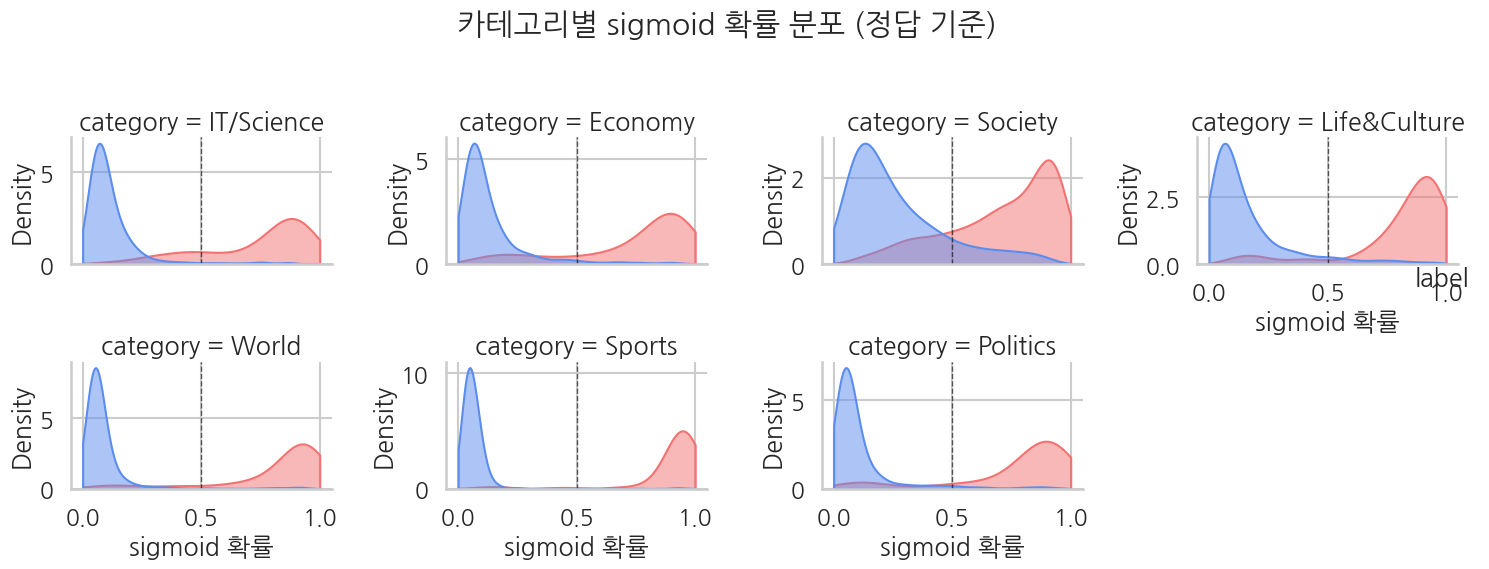
\includegraphics[width=0.90\linewidth]{assets/figures/ch17_label_probability_facets.png}
\end{bookfigurelabel}

\textbf{그림 읽기} --- 그림~\ref{fig:ch17-label-probability-facets}에서 다음 내용을 확인합니다: KLUE-YNAT 다중 라벨 카테고리별 sigmoid 확률 분포. 실행된 노트북에서 저장된 최신 plot 출력이므로, 코드에서 계산한 값이 어떤 평가 지점으로 이어지는지 바로 확인할 수 있습니다.



\textbf{해석}

\begin{itemize}
\tightlist
\item
  \textbf{잘 학습된 카테고리} (예: 스포츠): label=0 곡선은 0 근처, label=1 곡선은 1 근처에 있고 둘이 거의 만나지 않음. \emph{분리가 깨끗}.
\item
  \textbf{혼동하는 카테고리} (예: 사회 \(\leftrightarrow\) 생활문화 \(\leftrightarrow\) 정치): 두 곡선이 0.5 근처에서 크게 겹침. 결합 헤드라인 안에서 두 주제 신호가 \emph{섞이는} 카테고리.
\item
  \textbf{결합의 부작용} --- 한 샘플에 \emph{두 헤드라인} 이 들어가니 모델이 “둘 중 어느 쪽 신호가 어느 라벨인지” 분리해야 합니다. 이게 단일 헤드라인 (\ref{ch:16}장) 보다 어려운 점이고, multi-label task 의 자연스러운 난이도.
\end{itemize}



\subsection{카테고리 간 공동 활성 패턴}

Multi-label 의 핵심 질문: \emph{어떤 카테고리 쌍이 같이 등장하는가?} 합성 방식이 \emph{무작위 결합} 이라 true co-occurrence 는 거의 균등에 가까워야 하고, 모델 예측이 그 패턴을 따라가는지 확인합니다.

\inlinecode{true\ co-occurrence} (실제 합성 라벨의 동시 등장) 와 \inlinecode{predicted\ co-occurrence} (모델 예측의 동시 등장) 를 나란히 그립니다.



\compactCodeOmitted{숫자 결과를 그림으로 확인하는 단계}

\begin{bookfigurelabel}[H]{KLUE-YNAT 합성 다중 라벨의 공동 활성 행렬}{fig:ch17-cooccurrence}
\centering
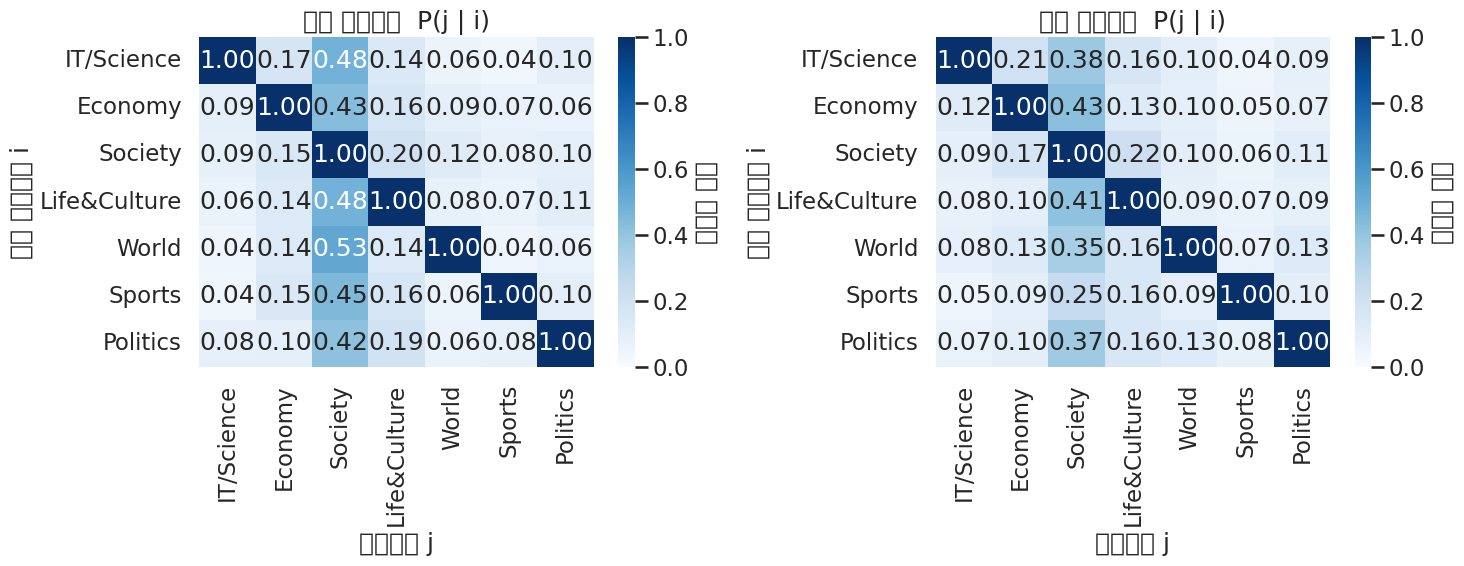
\includegraphics[width=0.92\linewidth]{assets/figures/ch17_cooccurrence.png}
\end{bookfigurelabel}

\textbf{그림 읽기} --- 그림~\ref{fig:ch17-cooccurrence}에서 다음 내용을 확인합니다: KLUE-YNAT 합성 다중 라벨의 공동 활성 행렬. 실행된 노트북에서 저장된 최신 plot 출력이므로, 코드에서 계산한 값이 어떤 평가 지점으로 이어지는지 바로 확인할 수 있습니다.



\textbf{해석}

\begin{itemize}
\tightlist
\item
  \textbf{대각선 = 1.0} --- 자기 자신과는 항상 같이 등장 (정의상).
\item
  \textbf{off-diagonal cell M{[}i, j{]}} = “카테고리 i 가 활성된 샘플 중 카테고리 j 도 활성된 비율”.
\item
  \textbf{합성이 무작위 결합} 이라 true 행렬의 off-diagonal 은 \emph{대략 균등} (각 카테고리의 전체 활성률에 비례) --- 특정 쌍이 \emph{유난히 높지 않음}. 실제 사람-annotated 데이터라면 “정치+경제” 처럼 \emph{자연스러운 상관} 이 드러나겠지만, 여기선 합성 방식 때문에 그런 구조가 약합니다.
\item
  \textbf{predicted cell 이 true 보다 일관되게 높으면} \(\to\) 모델이 라벨을 \emph{너무 많이} 활성하는 경향 (over-prediction). threshold 를 0.5 보다 높게 두면 calibration 개선.
\end{itemize}



\section{변형: 임계값 탐색}

결합 헤드라인을 \emph{문장 단위} 로 읽어보며 모델이 \emph{두 주제를 모두 잡는지} 확인합니다. 평가 metric 은 전체 평균이라 \emph{한 샘플에서 무슨 일이 일어나는지} 직관이 안 옵니다.



\Needspace{11\baselineskip}
\begin{lstlisting}
texts = list(eval_full["text"])
n_active_eval = labels.sum(axis=1)

two_active = np.where(n_active_eval == 2)[0]
hit_both, partial, conf_wrong = -1, -1, -1
best_conf_wrong = -1.0
for idx in two_active:
    match = (preds[idx] == labels[idx]).all()
    n_correct = int((preds[idx] * labels[idx]).sum())
    if match and hit_both < 0:
        hit_both = idx
    if (not match) and n_correct == 1 and partial < 0:
        partial = idx

\end{lstlisting}

\noindent\emph{앞뒤 블록은 모두 앞에서 만든 중간 값을 다음 계산으로 넘기는 단계입니다. 길이를 나누어 같은 흐름을 단계별로 확인합니다.}

\Needspace{11\baselineskip}
\begin{lstlisting}[firstnumber=15]
    wrong_pos = ((labels[idx] == 0) & (preds[idx] == 1))
    if wrong_pos.any():
        max_wrong = float(probs[idx][wrong_pos].max())
        if max_wrong > best_conf_wrong:
            best_conf_wrong, conf_wrong = max_wrong, idx

samples = [
    ("both categories correct", hit_both),
    ("partially correct (1 of 2)", partial),
    ("confidently wrong activation", conf_wrong),
]

\end{lstlisting}

\noindent\emph{앞뒤 블록은 모두 앞에서 만든 중간 값을 다음 계산으로 넘기는 단계입니다. 길이를 나누어 같은 흐름을 단계별로 확인합니다.}

\Needspace{11\baselineskip}
\begin{lstlisting}[firstnumber=27]
for label_kind, idx in samples:
    if idx < 0:
        continue
    print("=" * 80)
    print(f"sample #{idx}  ({label_kind})")
    print("=" * 80)
    print(f"text: {texts[idx]}")
    print()
    print(
        f"{'category':>10}  {'true':>5}  {'prob':>8}  "
        f"{'pred(>=0.5)':>12}  match"
    )
\end{lstlisting}

\noindent\emph{앞 블록은 앞에서 만든 중간 값을 다음 계산으로 넘기는 단계입니다. 이어지는 블록에서는 모델 출력을 확률이나 예측값으로 바꾸는 단계로 넘어갑니다.}

\Needspace{11\baselineskip}
\begin{lstlisting}[firstnumber=39]
    for k in range(K):
        t = int(labels[idx, k])
        p = float(probs[idx, k])
        pr = int(preds[idx, k])
        ok = "O" if t == pr else "X"
        print(
            f"  {LABEL_NAMES_EN[k]:>9}  {t:>5}  {p:>8.4f}  {pr:>12}    "
            f"{ok}"
        )
    true_active = [LABEL_NAMES_EN[k] for k in range(K) if labels[idx, k]]
    pred_active = [LABEL_NAMES_EN[k] for k in range(K) if preds[idx, k]]
    print()
    print(f"  true:      {true_active}")
    print(f"  predicted: {pred_active}")
    print()
\end{lstlisting}



\textbf{읽는 법}

\begin{itemize}
\tightlist
\item
  \textbf{\inlinecode{true} 컬럼} --- 합성 시 결합한 두 헤드라인의 카테고리. 보통 두 위치가 1.
\item
  \textbf{\inlinecode{prob} 컬럼} --- 각 카테고리 sigmoid 확률 (독립). 합이 1 일 필요 없음 --- multi-label 의 본질.
\item
  \textbf{\inlinecode{both\ categories\ correct}} --- 모델이 결합 헤드라인 안의 \emph{두 신호를 모두} 분리해 잡은 이상적 케이스.
\item
  \textbf{\inlinecode{partially\ correct}} --- 한 주제만 잡고 다른 하나는 놓침. 두 헤드라인 중 \emph{한쪽 신호가 약했거나} 두 카테고리가 서로 혼동하는 경우.
\item
  \textbf{\inlinecode{confidently\ wrong}} --- 정답이 0 인데 높은 확률로 활성. 결합된 두 헤드라인의 단어가 \emph{제3의 카테고리} 신호와 겹친 경우 (예: 경제+세계 헤드라인이 \textquotesingle 정치\textquotesingle{} 신호처럼 보임).
\end{itemize}



\compactCodeOmitted{예측 결과를 지표와 표로 요약하는 단계}

\begin{bookfigurelabel}[H]{KLUE-YNAT 다중 라벨 임계값 탐색}{fig:ch17-threshold-sweep}
\centering
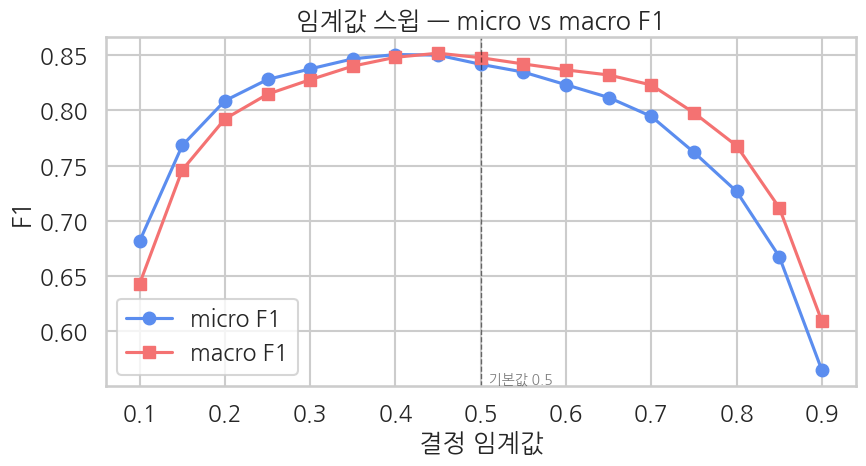
\includegraphics[width=0.86\linewidth]{assets/figures/ch17_threshold_sweep.png}
\end{bookfigurelabel}

\textbf{그림 읽기} --- 그림~\ref{fig:ch17-threshold-sweep}에서 다음 내용을 확인합니다: KLUE-YNAT 다중 라벨 임계값 탐색. 실행된 노트북에서 저장된 최신 plot 출력이므로, 코드에서 계산한 값이 어떤 평가 지점으로 이어지는지 바로 확인할 수 있습니다.



\textbf{해석} --- threshold 0.5 가 \emph{항상} 최적은 아닙니다. 활성률이 낮은 카테고리가 있으면 \emph{낮은 threshold} 가 recall 을 끌어올려 F1 이 더 좋아질 수 있습니다. 운영 단계에선 validation set 에서 \emph{카테고리별로} 최적 threshold 를 찾아 저장해 두고 추론 시 적용 (FAQ Q1).



\section{이 장에 등장한 라이브러리·함수}

\begin{booktable}{17장 새로 등장한 라이브러리}{tab:ch17-05}
\begin{adjustbox}{max width=\textwidth}
\begin{tabular}{@{}lll@{}}
\toprule
이름 & 한 줄 설명 & 다음 장에서 \\
\midrule

\inlinecode{AutoModelForSequenceClassification(num\_labels=7,\ problem\_type="multi\_label\_classification")} & \ref{ch:16}장 셋업에서 problem\_type 만 변경 \(\to\) BCE per-label 자동 매핑 & \ref{ch:18}장에서 메인 헤드로 그대로 \\
\inlinecode{datasets.Dataset.from\_dict(...)} & 합성한 텍스트·라벨로 새 데이터셋 생성 & 합성 데이터 장에서 재등장 \\
\inlinecode{numpy.random.default\_rng(seed)} & 재현 가능한 난수 생성기 (결합 짝짓기) & 합성 장마다 \\
\inlinecode{sklearn.metrics.hamming\_loss} & 전체 (sample \(\times\) label) 위치 중 틀린 비율 & multi-label 장마다 \\
\inlinecode{precision\_recall\_fscore\_support(...,\ average="micro"/"macro")} & multi-label F1 --- micro 는 라벨 합산, macro 는 라벨 평균 & \ref{ch:18}장 \\
\inlinecode{roc\_auc\_score(...,\ average="macro")} & 카테고리별 AUC 의 macro 평균 & \ref{ch:18}장 \\
\inlinecode{seaborn.FacetGrid\ +\ map\_dataframe} & 7개 카테고리에 같은 KDE 를 facet 으로 & 라벨이 많은 시각화에 재등장 \\
\bottomrule
\end{tabular}
\end{adjustbox}
\end{booktable}



\section{체크포인트 질문}

\begin{enumerate}
\def\labelenumi{\arabic{enumi}.}
\tightlist
\item
  \ref{ch:16}장과 \ref{ch:17}장의 모델이 \emph{둘 다} \inlinecode{Linear(H,\ 7)} 헤드인데, 같은 7개 출력을 두 장이 \emph{어떻게 다르게 해석} 하나요?
\item
  multi-label 문제를 \emph{softmax + CrossEntropyLoss} 로 풀려고 하면 무엇이 잘못되나요? 합성 샘플 (경제+스포츠) 을 예로 한 줄 설명할 수 있나요?
\item
  두 헤드라인을 \texttt{{[}SEP{]}} 로 잇는 합성 방식에서, 모델이 \emph{두 주제를 모두 잡지 못하고 하나만 잡는} 경우는 왜 생기나요?
\item
  카테고리 간 공동 활성 행렬에서 \emph{무작위 결합} 합성이라 true co-occurrence 가 거의 균등에 가까운데, 실제 사람-annotated multi-label 데이터라면 이 행렬이 어떻게 달라질까요?
\end{enumerate}



\section{FAQ}



\begin{faqBox}{Q3. (실무) \inlinecode{pos\_weight} 로 카테고리 불균형을 다루려면?}

\inlinecode{BCEWithLogitsLoss(pos\_weight=...)} 가 라벨별 양성 가중치를 받습니다. 무작위 결합이라 카테고리 활성률이 KLUE-YNAT 원본 분포를 따라가 \emph{약간 불균형} (스포츠/세계가 정치/IT 보다 많음).

\Needspace{11\baselineskip}
\begin{lstlisting}
import torch
from torch import nn

pos_count = Y_train.sum(axis=0)
neg_count = len(Y_train) - pos_count
pos_weight = torch.tensor(
    neg_count / np.maximum(pos_count, 1),
    dtype=torch.float,
)

\end{lstlisting}

\noindent\emph{앞 블록은 필요한 라이브러리와 기본 설정을 준비하는 단계입니다. 이어지는 블록에서는 학습 설정을 만들고 학습 루프를 실행하는 단계로 넘어갑니다.}

\Needspace{9\baselineskip}
\begin{lstlisting}[firstnumber=11]
class WeightedTrainer(Trainer):
    def compute_loss(self, model, inputs, return_outputs=False, **kwargs):
        labels = inputs.pop("labels")
        outputs = model(**inputs)
        loss_fn = nn.BCEWithLogitsLoss(pos_weight=pos_weight.to(outputs.logits.device))
        loss = loss_fn(outputs.logits, labels)
        return (loss, outputs) if return_outputs else loss
\end{lstlisting}

활성률이 낮은 카테고리는 pos\_weight 가 커져 양성 샘플의 손실이 더 가중됩니다 \(\to\) 모델이 그 카테고리를 더 자주 활성하도록.

\end{faqBox}



\begin{faqBox}{Q6. (이론) micro F1 과 macro F1 중 multi-label 에선 어느 쪽을 봐야 하나요?}

둘 다 봐야 하지만 보는 \emph{이유} 가 다릅니다.

\begin{itemize}
\tightlist
\item
  \textbf{micro F1} --- 모든 (샘플 \(\times\) 카테고리) 위치를 동등하게 세서 합산. \emph{활성률 높은 카테고리} 의 영향이 큼. “전체적으로 라벨을 얼마나 잘 맞히나” 의 종합 점수.
\item
  \textbf{macro F1} --- 카테고리 7개의 F1 을 \emph{단순 평균}. 활성률이 낮은 카테고리도 \emph{동등한 가중치}. “소수 카테고리도 챙기나” 의 공정성 점수.
\end{itemize}

micro 가 높은데 macro 가 \emph{훨씬} 낮으면 \(\to\) 모델이 \emph{다수 카테고리만 잘 맞히고 소수 카테고리를 버리는} 상태. 이때 Q3 의 \inlinecode{pos\_weight} 나 Q1 의 카테고리별 threshold 로 처치.

\end{faqBox}

\begin{faqBox}{Q7. (실무) 합성 multi-label 로 학습한 모델을 실제 multi-topic 뉴스에 써도 되나요?}

부분적으로 됩니다. 합성 데이터로도 모델은 \emph{각 카테고리의 단어·표현 신호} 를 학습하므로, 진짜 multi-topic 헤드라인에서도 \emph{기본적인 카테고리 인식} 은 작동합니다. 단 Q2 에서 짚은 한계 때문에:

\begin{itemize}
\tightlist
\item
  \emph{자연스러운 카테고리 상관} 을 못 배웠으니 “정치+경제 가 흔하다” 같은 사전 지식이 없음.
\item
  \emph{한 문장에 융합된} multi-topic (이어붙임이 아닌) 에는 약함.
\end{itemize}

실무에선 \emph{소량의 사람-annotated multi-label 데이터} 로 fine-tune 을 한 번 더 하면 (합성 \(\to\) 진짜 데이터 2단계) 격차가 크게 줄어듭니다. 합성 데이터의 가치는 \emph{없는 라벨을 0 에서 만드는 것} 이 아니라 \emph{모델을 task 형태에 적응시키는 워밍업} 에 있습니다.
\end{faqBox}



\compactFAQMore{4}

\section{오류 실험 (선택)}

다음 코드를 돌려보면 어떤 에러가 날까요?

\Needspace{11\baselineskip}
\begin{lstlisting}
def tokenize_wrong(batch):
    out = tokenizer(
        batch["text"],
        truncation=True,
        max_length=128,
    )

    out["labels"] = [
        next((i for i, v in enumerate(mh) if v > 0), 0)
        for mh in batch["multi_hot"]
    ]
    return out
\end{lstlisting}

힌트: \inlinecode{BCEWithLogitsLoss} 는 \emph{logits 와 같은 shape 의 float 텐서} 를 라벨로 받는데, 위 코드는 \emph{(B,) int} 를 넘깁니다. shape mismatch + dtype mismatch 두 가지 에러가 동시에 날 수 있어 메시지가 길어집니다 (\ref{ch:13}장의 삽질과 같은 함정 --- 라벨 \emph{형식} 이 problem\_type 과 일치해야 함).



\begin{previewBox}{미리보기: 다음 장}

\textbf{\ref{ch:18}장. 한국어 BERT Auxiliary Loss --- multi-label 분류 + 활성 라벨 개수 보조 회귀}

\begin{itemize}
\tightlist
\item
  메인 task: \ref{ch:17}장의 multi-label 카테고리 분류 (\inlinecode{num\_labels=7} + BCE per-label) --- \emph{완전히 동일}
\item
  추가: \emph{보조 헤드} \inlinecode{Linear(H,\ 1)} 로 \emph{활성 라벨 개수} 를 회귀 (결합한 헤드라인이 몇 개 카테고리에 걸치는가, 정규화 0-1)
\item
  손실: \texttt{L\ =\ BCE\_per\_label(메인)\ +\ λ\ ·\ MSE(보조)} 가중합 (\(\lambda\) 는 hyperparameter)
\item
  \inlinecode{Trainer.compute\_loss} 오버라이드로 두 헤드를 동시 학습
\item
  \ref{ch:14}장 (영어 auxiliary) 의 한국어 버전 --- 보조 task 만 별점 회귀 \(\to\) 라벨 개수 회귀로 달라짐
\end{itemize}

\begin{quote}
\textbf{변하는 축}: 메인 task 와 모델 본체는 그대로, \emph{Loss 에 보조 항이 추가} 됩니다 --- Loss 축의 마지막 단계 (“BCE per-label \(\to\) +Auxiliary”).
\end{quote}
\end{previewBox}